% Created by tikzDevice version 0.12.3.1 on 2022-05-11 21:42:37
% !TEX encoding = UTF-8 Unicode
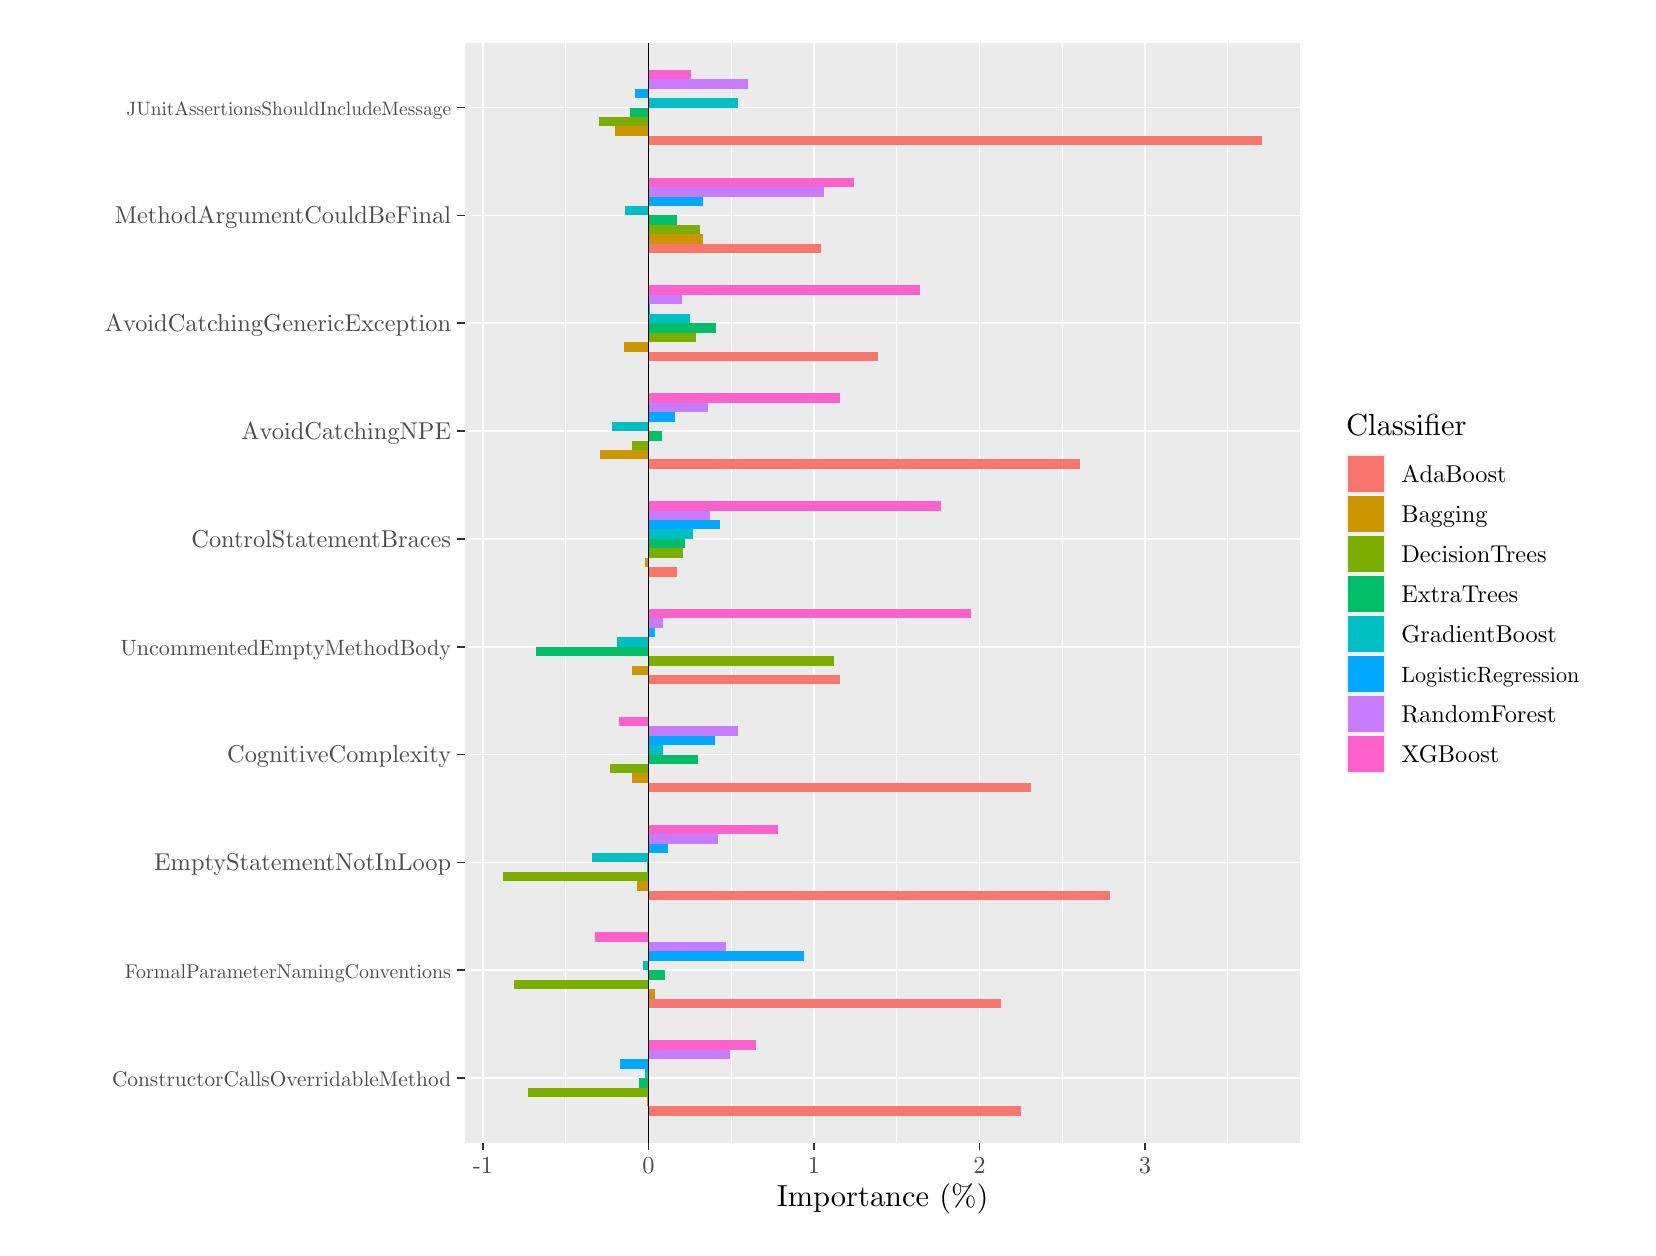
\begin{tikzpicture}[x=1pt,y=1pt]
\definecolor{fillColor}{RGB}{255,255,255}
\path[use as bounding box,fill=fillColor,fill opacity=0.00] (0,0) rectangle (578.16,433.62);
\begin{scope}
\path[clip] (  0.00,  0.00) rectangle (578.16,433.62);
\definecolor{drawColor}{RGB}{255,255,255}
\definecolor{fillColor}{RGB}{255,255,255}

\path[draw=drawColor,line width= 0.6pt,line join=round,line cap=round,fill=fillColor] (  0.00,  0.00) rectangle (578.16,433.62);
\end{scope}
\begin{scope}
\path[clip] (157.96, 30.69) rectangle (459.91,428.12);
\definecolor{fillColor}{gray}{0.92}

\path[fill=fillColor] (157.96, 30.69) rectangle (459.91,428.12);
\definecolor{drawColor}{RGB}{255,255,255}

\path[draw=drawColor,line width= 0.3pt,line join=round] (194.41, 30.69) --
	(194.41,428.12);

\path[draw=drawColor,line width= 0.3pt,line join=round] (254.21, 30.69) --
	(254.21,428.12);

\path[draw=drawColor,line width= 0.3pt,line join=round] (314.02, 30.69) --
	(314.02,428.12);

\path[draw=drawColor,line width= 0.3pt,line join=round] (373.82, 30.69) --
	(373.82,428.12);

\path[draw=drawColor,line width= 0.3pt,line join=round] (433.62, 30.69) --
	(433.62,428.12);

\path[draw=drawColor,line width= 0.6pt,line join=round] (157.96, 54.06) --
	(459.91, 54.06);

\path[draw=drawColor,line width= 0.6pt,line join=round] (157.96, 93.03) --
	(459.91, 93.03);

\path[draw=drawColor,line width= 0.6pt,line join=round] (157.96,131.99) --
	(459.91,131.99);

\path[draw=drawColor,line width= 0.6pt,line join=round] (157.96,170.96) --
	(459.91,170.96);

\path[draw=drawColor,line width= 0.6pt,line join=round] (157.96,209.92) --
	(459.91,209.92);

\path[draw=drawColor,line width= 0.6pt,line join=round] (157.96,248.88) --
	(459.91,248.88);

\path[draw=drawColor,line width= 0.6pt,line join=round] (157.96,287.85) --
	(459.91,287.85);

\path[draw=drawColor,line width= 0.6pt,line join=round] (157.96,326.81) --
	(459.91,326.81);

\path[draw=drawColor,line width= 0.6pt,line join=round] (157.96,365.78) --
	(459.91,365.78);

\path[draw=drawColor,line width= 0.6pt,line join=round] (157.96,404.74) --
	(459.91,404.74);

\path[draw=drawColor,line width= 0.6pt,line join=round] (164.51, 30.69) --
	(164.51,428.12);

\path[draw=drawColor,line width= 0.6pt,line join=round] (224.31, 30.69) --
	(224.31,428.12);

\path[draw=drawColor,line width= 0.6pt,line join=round] (284.12, 30.69) --
	(284.12,428.12);

\path[draw=drawColor,line width= 0.6pt,line join=round] (343.92, 30.69) --
	(343.92,428.12);

\path[draw=drawColor,line width= 0.6pt,line join=round] (403.72, 30.69) --
	(403.72,428.12);
\definecolor{fillColor}{RGB}{248,118,109}

\path[fill=fillColor] (224.31,391.10) rectangle (446.18,394.51);

\path[fill=fillColor] (224.31,352.14) rectangle (286.51,355.55);

\path[fill=fillColor] (224.31,313.18) rectangle (307.44,316.59);

\path[fill=fillColor] (224.31,274.21) rectangle (380.40,277.62);

\path[fill=fillColor] (224.31,235.25) rectangle (234.48,238.66);

\path[fill=fillColor] (224.31,196.28) rectangle (293.68,199.69);

\path[fill=fillColor] (224.31,157.32) rectangle (362.46,160.73);

\path[fill=fillColor] (224.31,118.36) rectangle (391.16,121.76);

\path[fill=fillColor] (224.31, 79.39) rectangle (351.69, 82.80);

\path[fill=fillColor] (224.31, 40.43) rectangle (358.87, 43.84);
\definecolor{fillColor}{RGB}{205,150,0}

\path[fill=fillColor] (212.35,394.51) rectangle (224.31,397.92);

\path[fill=fillColor] (224.31,355.55) rectangle (244.05,358.96);

\path[fill=fillColor] (215.34,316.59) rectangle (224.31,319.99);

\path[fill=fillColor] (206.97,277.62) rectangle (224.31,281.03);

\path[fill=fillColor] (223.12,238.66) rectangle (224.31,242.07);

\path[fill=fillColor] (218.33,199.69) rectangle (224.31,203.10);

\path[fill=fillColor] (218.33,160.73) rectangle (224.31,164.14);

\path[fill=fillColor] (220.13,121.76) rectangle (224.31,125.17);

\path[fill=fillColor] (224.31, 82.80) rectangle (226.71, 86.21);

\path[fill=fillColor] (223.71, 43.84) rectangle (224.31, 47.25);
\definecolor{fillColor}{RGB}{124,174,0}

\path[fill=fillColor] (206.37,397.92) rectangle (224.31,401.33);

\path[fill=fillColor] (224.31,358.96) rectangle (242.85,362.37);

\path[fill=fillColor] (224.31,319.99) rectangle (241.66,323.40);

\path[fill=fillColor] (218.33,281.03) rectangle (224.31,284.44);

\path[fill=fillColor] (224.31,242.07) rectangle (236.87,245.48);

\path[fill=fillColor] (224.31,203.10) rectangle (291.29,206.51);

\path[fill=fillColor] (210.56,164.14) rectangle (224.31,167.55);

\path[fill=fillColor] (171.69,125.17) rectangle (224.31,128.58);

\path[fill=fillColor] (175.87, 86.21) rectangle (224.31, 89.62);

\path[fill=fillColor] (180.66, 47.25) rectangle (224.31, 50.65);
\definecolor{fillColor}{RGB}{0,190,103}

\path[fill=fillColor] (217.73,401.33) rectangle (224.31,404.74);

\path[fill=fillColor] (224.31,362.37) rectangle (234.48,365.78);

\path[fill=fillColor] (224.31,323.40) rectangle (248.83,326.81);

\path[fill=fillColor] (224.31,284.44) rectangle (229.10,287.85);

\path[fill=fillColor] (224.31,245.48) rectangle (237.47,248.88);

\path[fill=fillColor] (183.65,206.51) rectangle (224.31,209.92);

\path[fill=fillColor] (224.31,167.55) rectangle (242.25,170.96);

\path[fill=fillColor] (223.71,128.58) rectangle (224.31,131.99);

\path[fill=fillColor] (224.31, 89.62) rectangle (230.29, 93.03);

\path[fill=fillColor] (220.72, 50.65) rectangle (224.31, 54.06);
\definecolor{fillColor}{RGB}{0,191,196}

\path[fill=fillColor] (224.31,404.74) rectangle (256.61,408.15);

\path[fill=fillColor] (215.94,365.78) rectangle (224.31,369.19);

\path[fill=fillColor] (224.31,326.81) rectangle (239.26,330.22);

\path[fill=fillColor] (211.16,287.85) rectangle (224.31,291.26);

\path[fill=fillColor] (224.31,248.88) rectangle (240.46,252.29);

\path[fill=fillColor] (212.95,209.92) rectangle (224.31,213.33);

\path[fill=fillColor] (224.31,170.96) rectangle (229.70,174.37);

\path[fill=fillColor] (203.98,131.99) rectangle (224.31,135.40);

\path[fill=fillColor] (222.52, 93.03) rectangle (224.31, 96.44);

\path[fill=fillColor] (223.12, 54.06) rectangle (224.31, 57.47);
\definecolor{fillColor}{RGB}{0,169,255}

\path[fill=fillColor] (219.53,408.15) rectangle (224.31,411.56);

\path[fill=fillColor] (224.31,369.19) rectangle (244.05,372.60);

\path[fill=fillColor] (224.31,330.22) rectangle (224.91,333.63);

\path[fill=fillColor] (224.31,291.26) rectangle (233.88,294.67);

\path[fill=fillColor] (224.31,252.29) rectangle (250.03,255.70);

\path[fill=fillColor] (224.31,213.33) rectangle (226.71,216.74);

\path[fill=fillColor] (224.31,174.37) rectangle (248.23,177.78);

\path[fill=fillColor] (224.31,135.40) rectangle (231.49,138.81);

\path[fill=fillColor] (224.31, 96.44) rectangle (280.53, 99.85);

\path[fill=fillColor] (214.15, 57.47) rectangle (224.31, 60.88);
\definecolor{fillColor}{RGB}{199,124,255}

\path[fill=fillColor] (224.31,411.56) rectangle (260.19,414.97);

\path[fill=fillColor] (224.31,372.60) rectangle (287.70,376.01);

\path[fill=fillColor] (224.31,333.63) rectangle (236.27,337.04);

\path[fill=fillColor] (224.31,294.67) rectangle (245.84,298.08);

\path[fill=fillColor] (224.31,255.70) rectangle (246.44,259.11);

\path[fill=fillColor] (224.31,216.74) rectangle (229.70,220.15);

\path[fill=fillColor] (224.31,177.78) rectangle (256.61,181.18);

\path[fill=fillColor] (224.31,138.81) rectangle (249.43,142.22);

\path[fill=fillColor] (224.31, 99.85) rectangle (252.42,103.26);

\path[fill=fillColor] (224.31, 60.88) rectangle (253.62, 64.29);
\definecolor{fillColor}{RGB}{255,97,204}

\path[fill=fillColor] (224.31,414.97) rectangle (239.86,418.38);

\path[fill=fillColor] (224.31,376.01) rectangle (298.47,379.41);

\path[fill=fillColor] (224.31,337.04) rectangle (322.39,340.45);

\path[fill=fillColor] (224.31,298.08) rectangle (293.68,301.49);

\path[fill=fillColor] (224.31,259.11) rectangle (330.16,262.52);

\path[fill=fillColor] (224.31,220.15) rectangle (340.93,223.56);

\path[fill=fillColor] (213.55,181.18) rectangle (224.31,184.59);

\path[fill=fillColor] (224.31,142.22) rectangle (270.96,145.63);

\path[fill=fillColor] (205.18,103.26) rectangle (224.31,106.67);

\path[fill=fillColor] (224.31, 64.29) rectangle (263.19, 67.70);
\definecolor{drawColor}{RGB}{0,0,0}

\path[draw=drawColor,line width= 0.6pt,line join=round] (224.31, 30.69) -- (224.31,428.12);
\end{scope}
\begin{scope}
\path[clip] (  0.00,  0.00) rectangle (578.16,433.62);
\definecolor{drawColor}{gray}{0.30}

\node[text=drawColor,anchor=base east,inner sep=0pt, outer sep=0pt, scale=  0.77] at (153.01, 51.03) {ConstructorCallsOverridableMethod};

\node[text=drawColor,anchor=base east,inner sep=0pt, outer sep=0pt, scale=  0.72] at (153.01, 90.00) {FormalParameterNamingConventions};

\node[text=drawColor,anchor=base east,inner sep=0pt, outer sep=0pt, scale=  0.88] at (153.01,128.96) {EmptyStatementNotInLoop};

\node[text=drawColor,anchor=base east,inner sep=0pt, outer sep=0pt, scale=  0.88] at (153.01,167.93) {CognitiveComplexity};

\node[text=drawColor,anchor=base east,inner sep=0pt, outer sep=0pt, scale=  0.80] at (153.01,206.89) {UncommentedEmptyMethodBody};

\node[text=drawColor,anchor=base east,inner sep=0pt, outer sep=0pt, scale=  0.88] at (153.01,245.85) {ControlStatementBraces};

\node[text=drawColor,anchor=base east,inner sep=0pt, outer sep=0pt, scale=  0.88] at (153.01,284.82) {AvoidCatchingNPE};

\node[text=drawColor,anchor=base east,inner sep=0pt, outer sep=0pt, scale=  0.88] at (153.01,323.78) {AvoidCatchingGenericException};

\node[text=drawColor,anchor=base east,inner sep=0pt, outer sep=0pt, scale=  0.88] at (153.01,362.75) {MethodArgumentCouldBeFinal};

\node[text=drawColor,anchor=base east,inner sep=0pt, outer sep=0pt, scale=  0.70] at (153.01,401.71) {JUnitAssertionsShouldIncludeMessage};
\end{scope}
\begin{scope}
\path[clip] (  0.00,  0.00) rectangle (578.16,433.62);
\definecolor{drawColor}{gray}{0.20}

\path[draw=drawColor,line width= 0.6pt,line join=round] (155.21, 54.06) --
	(157.96, 54.06);

\path[draw=drawColor,line width= 0.6pt,line join=round] (155.21, 93.03) --
	(157.96, 93.03);

\path[draw=drawColor,line width= 0.6pt,line join=round] (155.21,131.99) --
	(157.96,131.99);

\path[draw=drawColor,line width= 0.6pt,line join=round] (155.21,170.96) --
	(157.96,170.96);

\path[draw=drawColor,line width= 0.6pt,line join=round] (155.21,209.92) --
	(157.96,209.92);

\path[draw=drawColor,line width= 0.6pt,line join=round] (155.21,248.88) --
	(157.96,248.88);

\path[draw=drawColor,line width= 0.6pt,line join=round] (155.21,287.85) --
	(157.96,287.85);

\path[draw=drawColor,line width= 0.6pt,line join=round] (155.21,326.81) --
	(157.96,326.81);

\path[draw=drawColor,line width= 0.6pt,line join=round] (155.21,365.78) --
	(157.96,365.78);

\path[draw=drawColor,line width= 0.6pt,line join=round] (155.21,404.74) --
	(157.96,404.74);
\end{scope}
\begin{scope}
\path[clip] (  0.00,  0.00) rectangle (578.16,433.62);
\definecolor{drawColor}{gray}{0.20}

\path[draw=drawColor,line width= 0.6pt,line join=round] (164.51, 27.94) --
	(164.51, 30.69);

\path[draw=drawColor,line width= 0.6pt,line join=round] (224.31, 27.94) --
	(224.31, 30.69);

\path[draw=drawColor,line width= 0.6pt,line join=round] (284.12, 27.94) --
	(284.12, 30.69);

\path[draw=drawColor,line width= 0.6pt,line join=round] (343.92, 27.94) --
	(343.92, 30.69);

\path[draw=drawColor,line width= 0.6pt,line join=round] (403.72, 27.94) --
	(403.72, 30.69);
\end{scope}
\begin{scope}
\path[clip] (  0.00,  0.00) rectangle (578.16,433.62);
\definecolor{drawColor}{gray}{0.30}

\node[text=drawColor,anchor=base,inner sep=0pt, outer sep=0pt, scale=  0.88] at (164.51, 19.68) {-1};

\node[text=drawColor,anchor=base,inner sep=0pt, outer sep=0pt, scale=  0.88] at (224.31, 19.68) {0};

\node[text=drawColor,anchor=base,inner sep=0pt, outer sep=0pt, scale=  0.88] at (284.12, 19.68) {1};

\node[text=drawColor,anchor=base,inner sep=0pt, outer sep=0pt, scale=  0.88] at (343.92, 19.68) {2};

\node[text=drawColor,anchor=base,inner sep=0pt, outer sep=0pt, scale=  0.88] at (403.72, 19.68) {3};
\end{scope}
\begin{scope}
\path[clip] (  0.00,  0.00) rectangle (578.16,433.62);
\definecolor{drawColor}{RGB}{0,0,0}

\node[text=drawColor,anchor=base,inner sep=0pt, outer sep=0pt, scale=  1.10] at (308.93,  7.64) {Importance (\%)};
\end{scope}
\begin{scope}
\path[clip] (  0.00,  0.00) rectangle (578.16,433.62);
\definecolor{fillColor}{RGB}{255,255,255}

\path[fill=fillColor] (470.91,158.48) rectangle (572.66,300.33);
\end{scope}
\begin{scope}
\path[clip] (  0.00,  0.00) rectangle (578.16,433.62);
\definecolor{drawColor}{RGB}{0,0,0}

\node[text=drawColor,anchor=base west,inner sep=0pt, outer sep=0pt, scale=  1.10] at (476.41,286.18) {Classifier};
\end{scope}
\begin{scope}
\path[clip] (  0.00,  0.00) rectangle (578.16,433.62);
\definecolor{fillColor}{gray}{0.95}

\path[fill=fillColor] (476.41,265.16) rectangle (490.86,279.61);
\end{scope}
\begin{scope}
\path[clip] (  0.00,  0.00) rectangle (578.16,433.62);
\definecolor{fillColor}{RGB}{248,118,109}

\path[fill=fillColor] (477.12,265.87) rectangle (490.15,278.90);
\end{scope}
\begin{scope}
\path[clip] (  0.00,  0.00) rectangle (578.16,433.62);
\definecolor{fillColor}{gray}{0.95}

\path[fill=fillColor] (476.41,250.70) rectangle (490.86,265.16);
\end{scope}
\begin{scope}
\path[clip] (  0.00,  0.00) rectangle (578.16,433.62);
\definecolor{fillColor}{RGB}{205,150,0}

\path[fill=fillColor] (477.12,251.42) rectangle (490.15,264.45);
\end{scope}
\begin{scope}
\path[clip] (  0.00,  0.00) rectangle (578.16,433.62);
\definecolor{fillColor}{gray}{0.95}

\path[fill=fillColor] (476.41,236.25) rectangle (490.86,250.70);
\end{scope}
\begin{scope}
\path[clip] (  0.00,  0.00) rectangle (578.16,433.62);
\definecolor{fillColor}{RGB}{124,174,0}

\path[fill=fillColor] (477.12,236.96) rectangle (490.15,249.99);
\end{scope}
\begin{scope}
\path[clip] (  0.00,  0.00) rectangle (578.16,433.62);
\definecolor{fillColor}{gray}{0.95}

\path[fill=fillColor] (476.41,221.80) rectangle (490.86,236.25);
\end{scope}
\begin{scope}
\path[clip] (  0.00,  0.00) rectangle (578.16,433.62);
\definecolor{fillColor}{RGB}{0,190,103}

\path[fill=fillColor] (477.12,222.51) rectangle (490.15,235.54);
\end{scope}
\begin{scope}
\path[clip] (  0.00,  0.00) rectangle (578.16,433.62);
\definecolor{fillColor}{gray}{0.95}

\path[fill=fillColor] (476.41,207.34) rectangle (490.86,221.80);
\end{scope}
\begin{scope}
\path[clip] (  0.00,  0.00) rectangle (578.16,433.62);
\definecolor{fillColor}{RGB}{0,191,196}

\path[fill=fillColor] (477.12,208.05) rectangle (490.15,221.08);
\end{scope}
\begin{scope}
\path[clip] (  0.00,  0.00) rectangle (578.16,433.62);
\definecolor{fillColor}{gray}{0.95}

\path[fill=fillColor] (476.41,192.89) rectangle (490.86,207.34);
\end{scope}
\begin{scope}
\path[clip] (  0.00,  0.00) rectangle (578.16,433.62);
\definecolor{fillColor}{RGB}{0,169,255}

\path[fill=fillColor] (477.12,193.60) rectangle (490.15,206.63);
\end{scope}
\begin{scope}
\path[clip] (  0.00,  0.00) rectangle (578.16,433.62);
\definecolor{fillColor}{gray}{0.95}

\path[fill=fillColor] (476.41,178.43) rectangle (490.86,192.89);
\end{scope}
\begin{scope}
\path[clip] (  0.00,  0.00) rectangle (578.16,433.62);
\definecolor{fillColor}{RGB}{199,124,255}

\path[fill=fillColor] (477.12,179.15) rectangle (490.15,192.18);
\end{scope}
\begin{scope}
\path[clip] (  0.00,  0.00) rectangle (578.16,433.62);
\definecolor{fillColor}{gray}{0.95}

\path[fill=fillColor] (476.41,163.98) rectangle (490.86,178.43);
\end{scope}
\begin{scope}
\path[clip] (  0.00,  0.00) rectangle (578.16,433.62);
\definecolor{fillColor}{RGB}{255,97,204}

\path[fill=fillColor] (477.12,164.69) rectangle (490.15,177.72);
\end{scope}
\begin{scope}
\path[clip] (  0.00,  0.00) rectangle (578.16,433.62);
\definecolor{drawColor}{RGB}{0,0,0}

\node[text=drawColor,anchor=base west,inner sep=0pt, outer sep=0pt, scale=  0.88] at (496.36,269.35) {AdaBoost};
\end{scope}
\begin{scope}
\path[clip] (  0.00,  0.00) rectangle (578.16,433.62);
\definecolor{drawColor}{RGB}{0,0,0}

\node[text=drawColor,anchor=base west,inner sep=0pt, outer sep=0pt, scale=  0.88] at (496.36,254.90) {Bagging};
\end{scope}
\begin{scope}
\path[clip] (  0.00,  0.00) rectangle (578.16,433.62);
\definecolor{drawColor}{RGB}{0,0,0}

\node[text=drawColor,anchor=base west,inner sep=0pt, outer sep=0pt, scale=  0.88] at (496.36,240.45) {DecisionTrees};
\end{scope}
\begin{scope}
\path[clip] (  0.00,  0.00) rectangle (578.16,433.62);
\definecolor{drawColor}{RGB}{0,0,0}

\node[text=drawColor,anchor=base west,inner sep=0pt, outer sep=0pt, scale=  0.88] at (496.36,225.99) {ExtraTrees};
\end{scope}
\begin{scope}
\path[clip] (  0.00,  0.00) rectangle (578.16,433.62);
\definecolor{drawColor}{RGB}{0,0,0}

\node[text=drawColor,anchor=base west,inner sep=0pt, outer sep=0pt, scale=  0.88] at (496.36,211.54) {GradientBoost};
\end{scope}
\begin{scope}
\path[clip] (  0.00,  0.00) rectangle (578.16,433.62);
\definecolor{drawColor}{RGB}{0,0,0}

\node[text=drawColor,anchor=base west,inner sep=0pt, outer sep=0pt, scale=  0.80] at (496.36,197.08) {LogisticRegression};
\end{scope}
\begin{scope}
\path[clip] (  0.00,  0.00) rectangle (578.16,433.62);
\definecolor{drawColor}{RGB}{0,0,0}

\node[text=drawColor,anchor=base west,inner sep=0pt, outer sep=0pt, scale=  0.88] at (496.36,182.63) {RandomForest};
\end{scope}
\begin{scope}
\path[clip] (  0.00,  0.00) rectangle (578.16,433.62);
\definecolor{drawColor}{RGB}{0,0,0}

\node[text=drawColor,anchor=base west,inner sep=0pt, outer sep=0pt, scale=  0.88] at (496.36,168.18) {XGBoost};
\end{scope}
\end{tikzpicture}
